% -*- latex -*-
%%%%%%%%%%%%%%%%%%%%%%%%%%%%%%%%%%%%%%%%%%%%%%%%%%%%%%%%%%%%%%%%
%%%%%%%%%%%%%%%%%%%%%%%%%%%%%%%%%%%%%%%%%%%%%%%%%%%%%%%%%%%%%%%%
%%%%
%%%% This text file is part of the source of 
%%%% 'Parallel techniques'
%%%% by Ángel de Vicente, copyright 2019
%%%%
%%%% TO DO:
%%%%
%%%% intermediate-fortran.tex : intermediate fortran towards a
%%%%      Barnes-Hut N-body implementation
%%%% 
%%%%%%%%%%%%%%%%%%%%%%%%%%%%%%%%%%%%%%%%%%%%%%%%%%%%%%%%%%%%%%%%
%%%%%%%%%%%%%%%%%%%%%%%%%%%%%%%%%%%%%%%%%%%%%%%%%%%%%%%%%%%%%%%%

In order to implement the Barnes-Hut algorithm described in chapter
\ref{ch:barnes-hut.tex} we will need to learn some intermediate programming
concepts.

\Level 0 {Procedures and recursion}
\includepdf[frame=true,scale=0.98,pages={2-12,18-19}]{graphics/procedures_recursivity.pdf}

\Level 0 {Recursion exercises}
\label{sec:recursion-exercises}

\begin{verbatim}

1) Write a recursive function to calculate the Fibonacci numbers
 (https://en.wikipedia.org/wiki/Fibonacci_number)

2) Write a non-recursive version of the function above and compare the execution
 times of both versions for larger 'n' values (for example from 30-45). In Linux
 you can check the execution time with the command 'time' (for example: "time
 ./fibo_r 30").

3) Most probably, your recursive implementation is much slower than the
 iterative version. Can you guess what is going on? [Modify the recursive
 routine to count the number of times that the fibonacci function is
 called. Then, look for information on "memoization" and try to modify the
 recursive routine so that you still use recursion, but in a way that it is as
 efficient as the iterative version.

4) Write pseudo-code, that is, without paying attention to the syntax of
 Fortran, a recursive function to print in ascending order a Binary Search Tree
 (https://en.wikipedia.org/wiki/Binary_search_tree). You can assume that your
 function will be given a tree estructure called "tree", and that these
 functions are provided to you: left_branch_exists(tree), which will return TRUE
 is "tree" has a left branch, right_branch_exists(tree), left_branch(tree),
 which will return the left branch of the tree, right_branch(tree), and
 node_value(tree), which will return the value stored in the root node of the
 tree "tree".

5) Try to solve the Tower of Hanoi game:
 https://en.wikipedia.org/wiki/Tower_of_Hanoi

 This is more difficult than the previous exercises, but it shows very nicely how
 useful recursion is in some cases. You assume that you have a pile of pieces
 (the code should work for any number of pieces) in column 1 and you want to
 move them to column 3. As for the previous exercise, start with just
 pseudo-code, so you can concentrate on the problem while forgetting about the
 details of Fortran. But this one is perfectly doable with the little Fortran we
 have learnt so far, so you could try to go for a full implementation.

 In the page https://www.mathsisfun.com/games/towerofhanoi.html you can see a
 demonstration of how to solve the puzzle and you can try to solve it by hand. A
 basic implementation to solve this problem is very easy, just needing a routine
 that prints the necessary movements to solve the puzzle (we do not need to
 store the state of the puzzle at all, only print the moves that would solve the
 game. When executing the code, we could just print the number of moves, where
 each move has the following format:

 n (f -> t)

 where n is the piece number to move (1 is the smalles piece), f is the column
 whence the piece is coming, and t is the column where the piece is going
 to. For example:

$ ./hanoi
 Enter number of pieces
3
           1 (           1  ->            3 )
           2 (           1  ->            2 )
           1 (           3  ->            2 )
           3 (           1  ->            3 )
           1 (           2  ->            1 )
           2 (           2  ->            3 )
           1 (           1  ->            3 )

$ ./hanoi
 Enter number of pieces
4
           1 (           1  ->            2 )
           2 (           1  ->            3 )
           1 (           2  ->            3 )
           3 (           1  ->            2 )
           1 (           3  ->            1 )
           2 (           3  ->            2 )
           1 (           1  ->            2 )
           4 (           1  ->            3 )
           1 (           2  ->            3 )
           2 (           2  ->            1 )
           1 (           3  ->            1 )
           3 (           2  ->            3 )
           1 (           1  ->            2 )
           2 (           1  ->            3 )
           1 (           2  ->            3 )

6) In section 2.2.7, we looked at the Travelling Salesman Problem, but fixing it
 at 5 cities. Think about (and if possible implement) a recursive version that
 would work for any number of cities. If you understand how to write this one,
 then you are doing fantastic progress with recursion, as it gets a bit tricky
 to keep track of visited cities. If you don't get it at all, don't panic, we
 will see a solution in class.
\end{verbatim}


\Level 0 {Pointers and derived types}
{\includepdf[frame=true,scale=0.98,pages={2-21}]{graphics/pointers_derived_types.pdf}}

\Level 0 {Pointers exercises}
\label{sec:pointers-exercises}

\Level 0 {Pointers and recursion exercises}
\label{sec:pointers-recursion-exercises}



